\section{Лекция от 01.11.2016}

\subsection{Взаимно-однозначное соответствие функции распределения и вероятностной меры}
\begin{definition}
	Пусть функция $ F(x), x \in \R $, удовлетворяет свойствам из леммы, то есть: 
	\begin{enumerate}
		\item
		$F(x)$ неубывающая;
		\item
		\(\lim\limits_{x\to +\infty} F(x)= 1;\)
		\item
		\(\lim\limits_{x\to -\infty} F(x)= 0;\)
		\item
		$F(x)$ непрерывна справа.
	\end{enumerate}   
	Тогда такую функцию будем называть \emph{функцией распределения} на прямой.
\end{definition}

Следующая фундаментальная и очень важная теорема будет введена без доказательства.

\begin{theorem}[Теорема Каратеодори о продолжении меры]
	Пусть $ \Omega $ --- некоторое множество, $ \A $ -- алгебра подмножеств $ \Omega $. Пусть вероятностная мера \(\Pr_0: \A \mapsto [0; 1] \) удовлетворяет следующим свойствам:
	\begin{enumerate}
		\item
		\( \Pr_0(\Omega) = 1;  \)
		\item 
		\( \Pr_0 \) --- счетно-аддитивна на \(\A \).
	\end{enumerate}     
	Тогда существует (и притом единственна) вероятностная мера $ \Pr $ на $ \sigma(\A) $ такая, что мера $ \Pr $ является продолжением меры $ \Pr_0 $, иными словами \(\forall A \in \A \ \Pr_0(\A) = \Pr(\A)   \).
\end{theorem}

\begin{theorem}[Взаимно-однозначное соответствие функций распределения и мер на прямой]
	Пусть \(F(x), x \in \R \) --- функция распределения на прямой. Тогда существует (и притом единственна) вероятностная мера $ \Pr $ на \(\mathcal{B} \), такая что $ F(x) $ --- её функция распределения, то есть \(\forall x \in \R \ \Pr\left((-\infty; x] \right) = F(x) \).
\end{theorem}

\begin{proof}
	Рассмотрим алгебру $ \A $, состоящую из конечных объединений непересекающихся полуинтервалов вида \((a; b],\ \forall A \in \A \) имеет вид 
	\[
	\A = \bigcup\limits_{k=1}^{n}(a_k; b_k],\  -\infty \leq a_1 < b_1 < a_2 < b_2 < \ldots < b_n \leq +\infty.
	\]    
	Зададим на $ \A $ меру $ \Pr_0 $ по правилу 
	\[
	\Pr_0(\A) = \sum\limits_{k = 1}^{n}\left( F(b_k) - F(a_k)\right).    
	\] 
	Тогда \(\Pr_0(\R) = F(+\infty) - F(-\infty) = 1 - 0 = 1 \) и по построению $ \Pr_0 $ будет конечно-аддитивной мерой.
	
	Для того чтобы воспользоваться теоремой Каратеодори, вероятностная мера $ \Pr_0 $ должна обладать свойством счетной аддитивности. Но вместо того, чтобы доказывать это свойство напрямую, воспользуемся \emph{теоремой о непрерывности вероятностной меры} из предыдущей лекции и докажем эквивалентное условие. Покажем, что мера $ \Pr_0 $ является непрерывной в нуле.
	
	Итак, нужно проверить, выполняется ли
	\[
	\lim\limits_{n \to \infty}\Pr_0(A_n) = 0
	\]
	для любых множеств \(A_1, A_2, \ldots \in \A \) таких, что \(A_{n + 1} \subset A_n,\ \bigcap\limits_{n = 1}^{\infty}A_n = \emptyset \)
	
	Заметим, что для любого полуинтервала $ (a, b] $ и для любого $ \delta > 0 $ можно взять такое $ a' > a $, что: 
	\[
	\Pr_0\left((a; b] \right) - \Pr_0\left((a'; b]\right) \leq \delta
	\]  
	\[
	\Pr_0\left((a; b] \right) - \Pr_0\left((a'; b]\right) = \left(F(b) - F(a)\right) - \left(F(b) - F(a') \right) = F(a') - F(a). 
	\]
	
	Зафиксируем произольное $ \epsilon > 0 $.
	В силу непрерывности справа такое значение $ a' $ можно подобрать.
	Тогда 
	\[
	\forall A_n \exists B_n \in \A, такое что \Pr_0(A_n) - \Pr_0(B_n) \leq \epsilon2^{-n},\ B_n \in A_n \textbf{ и } [B_n] \in A_n, \text { где } [B_n] \text { есть замыкание } B_n. 
	\]
    То есть если $ B_n $ имеет вид $ (a, b] $, то $ [B_n] $, являющееся замыканием $ B_n $, имеет вид $ [a, b] $. Мы добавили в множество $ B_n $ его граничные точки.
	
	Пусть сначала все $ A_n $ лежат внутри $ [-N; N] $ для некоторого $ N \in \N $. Мы знаем, что \(\bigcap\limits_{n=1}^{\infty}A_n = \emptyset. \) Следовательно, \(\bigcap\limits_{n=1}^{\infty}[B_n] = \emptyset. \) 
	
	По принципу компактности существует $ n_0 $ такой, что из \(\bigcap\limits_{n=1}^{n_0}[B_n] = \emptyset \) следует \(\bigcap\limits_{n=1}^{n_0}B_n = \emptyset. \) Тогда:
	\[
	\Pr_0(A_{n_0}) = \Pr_0\left(A_{n_0} \setminus \bigcap\limits_{n=1}^{n_0}B_n\right)
	\]
	
	Следующий переход основан на том, что если \(\omega \in \A_n \setminus \bigcap\limits_{n=1}^{n_0}B_n \), то существует такой номер $ k $, что \(\omega \notin B_k\), а значит \(\omega \in \A_{n_0} \setminus B_k \).
	
	\begin{multline*} 
	\Pr_0\left(A_{n_0} \setminus \bigcap\limits_{n=1}^{n_0}B_n\right)
	\leq \sum\limits_{k=1}^{n_0}\Pr_0\left(A_{n_0} \setminus B_k \right) \leq \sum\limits_{k=1}^{n_0} \Pr_0\left(A_k \setminus B_k \right) \leq \\ \leq
	\sum\limits_{k=1}^{n_0} \left( \Pr_0\left(A_k\right) - \Pr_0\left(b_k\right) \right) \leq 
	\sum\limits_{k=1}^{n_0}\epsilon2^{-k} \leq \epsilon.
	\end{multline*}
	
	Получили, что \(\Pr_0(A_{n_0}) \leq \epsilon\). Значит, 
	\[
	\forall n > n_0 \ \Pr_0(A_n) \leq \epsilon \implies  \lim\limits_{n \to \infty}\Pr_0(A_n) = 0.
	\]
	
	Если в $ A_1 $ есть бесконечные полуинтервалы, то выберем полуинтервал $ (-N; N] $, что \(\Pr_0\left((-N; N] \right) \geq 1 - \frac{\epsilon}{2}\) и рассмотрим \(A_n' = A_n \cap (-N; N].  \)
	
	По доказанному выше \(\Pr_0(A_n') \leq \frac{\epsilon}{2} \) при $ n > n_0(\epsilon) $ и 
	\[
	\Pr_0(A_n) = \Pr_0\left(A_n' \cup \left(A_n \cup (-\infty; -N] \right) \cup \left(A_n \cap (N; +\infty)  \right)  \right) \leq \Pr_0\left(A_n'\right) + \Pr_0\left(\R \setminus (-N; N] \right) \leq \epsilon.
	\]
	
	По теореме Каратеодори искомая $ \Pr $ существует и единственна.
\end{proof}

\subsection{Классификация функций распределения на $\R$}

\subsubsection{Дискретные функции распределения}

    Вероятностная мера $\Pr$ на $\mathcal{B}(\R)$ называется дискретной, если $\exists X = \left\{ x_n
    \right\}$ --- не более чем счётное множество, такое что $\Pr{\R \setminus X} = 0$ и $\forall x_n \in X,
    \Pr{x_n} > 0$. Между прочим, в этом случае говорят, что $\Pr$ \emph{сосредоточена} в $X$.

    Но нас интересует функция распределения. Она будет выглядеть так:

    \[
        F(x) = \Pr{(-\infty, x]} = \sum\limits_{k: x_k \in X} \Pr{x_k}
    \]

    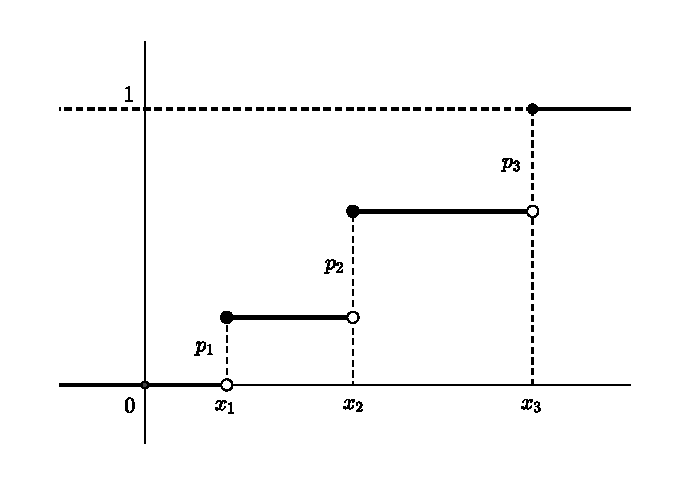
\includegraphics[width=15cm]{main-lectures/images/Lec_8_1.pdf}

    Примеры:

    \begin{itemize}
        \item Равномерное дискретное распределение:
            \[
                x = \left\{ 1\ldots n \right\}, \Pr_k = \frac{1}{n}
            \]

        \item Распределение Бернулли:
            \[
                x = \left\{ 0, 1 \right\}, \Pr_1 = p, \Pr_0 = 1-p
            \]
        \item Биномиальное распределение:
            \[
                \Pr_k = \binom{n}{k}p^k(1-p)^{n-k}
            \]
        \item Пуассоновское распределение:
            \[
                \Pr_k = \frac{\lambda^k}{k!}e^{-\lambda}
            \]
    \end{itemize}

\subsubsection{Абсолютно непрерывные функции распределения}

    Рассмотрим некоторую функцию $p(t)$, неотрицательную на $\R$, такую, что
    $\int\limits_{-\infty}^{\infty} p(t)dt = 1$.

    \begin{definition}
        Функция распределения $F(x)$ называется абсолютно непрерывной с плотностью $p(t)$, если $\forall x
        \in \R, F(x) = \int\limits_{-\infty}^{x} p(t)dt$
    \end{definition}

    Примеры:

    \begin{itemize}
        \item Равномерное распределение на отрезке:
            \[
                p(x) =
                \begin{cases}
                    \frac{1}{b-a}, &x \in [a, b]\\
                    0, &x \not\in [a, b]
                \end{cases}
            \]
            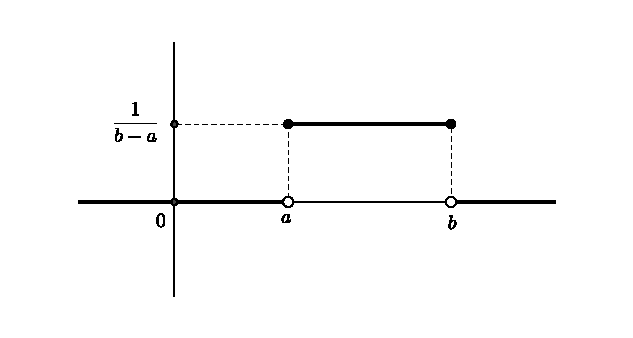
\includegraphics[width=13cm]{main-lectures/images/Lec_8_2.pdf}
            \[
                F(x) =
                \begin{cases}
                    0, &x < a\\
                    \frac{x-a}{b-a}, &x \in [a, b]\\
                    1, &x > b
                \end{cases}
            \]
            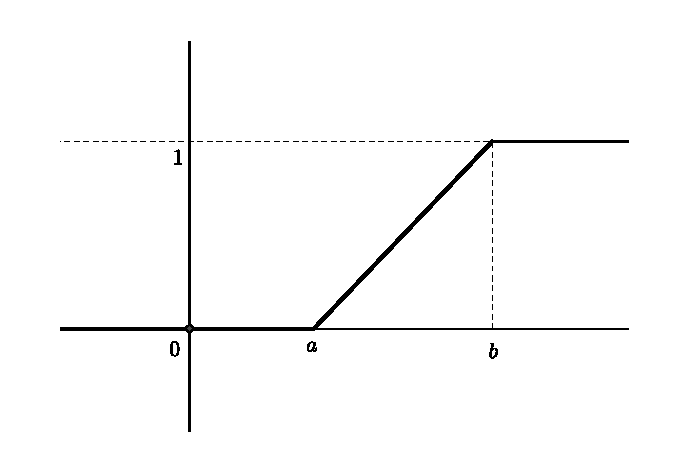
\includegraphics[width=12cm]{main-lectures/images/Lec_8_3.pdf}

        \item Нормальное распределение: $N(a, \sigma^2)$. Самое известное и распространённое распределение,
            встречающееся всюду; например погрешности измерений, как правило, подчиняются этому распределению.

            \[
                p(x) = \frac{1}{\sqrt{2\pi\sigma^2}}e^{-\frac{(x-a)^2}{2\sigma^2}}
            \]

            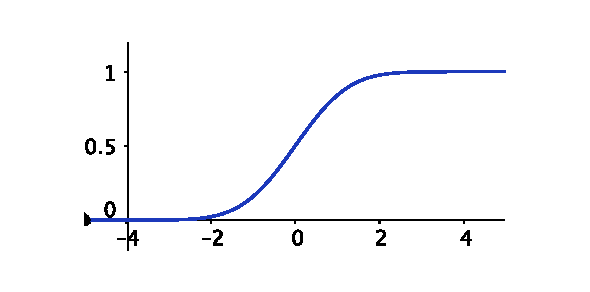
\includegraphics[width=12cm]{main-lectures/images/Lec_8_4.pdf}

            \[
                F(x) = \Phi\left(\frac{x - a}{\sigma}\right), \text{где $\Phi(x)$ --- функция Лапласа}
            \]

            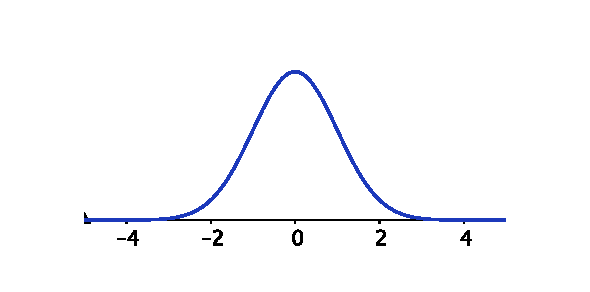
\includegraphics[width=12cm]{main-lectures/images/Lec_8_5.pdf}

        \item Экспоненциальное распределение: $\mathrm{Exp}(\alpha)$.

            \[
                p(x) = \begin{cases}
                    \alpha e^{-\alpha x}, &x > 0 \\
                    0, & otherwise
                    \end{cases}
            \]

            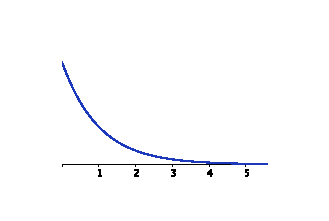
\includegraphics[width=12cm]{main-lectures/images/Lec_8_6.pdf}

            \[
                F(x) = \begin{cases}
                    1-e^{-\alpha x}, &x > 0\\
                    0, &x \leq 0
                \end{cases}
            \]

            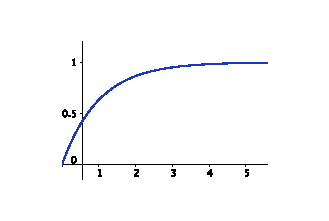
\includegraphics[width=12cm]{main-lectures/images/Lec_8_7.pdf}
    \end{itemize}

\subsubsection{Сингулярные функции распределения}

\begin{definition}
    Точка $y$ называется точкой роста функции $F(x), x \in \R$, если $\forall \epsilon > 0, F(y+\epsilon) -
    F(y - \epsilon) > 0$.
\end{definition}

\begin{definition}
    $\mathcal{A} \subset \R$ имеет Лебегову меру 0, если $\forall \epsilon$ существует набор интервалов
    $(a_n; b_n)$ таких что $\sum(b_k - a_k) < \epsilon$ и $\mathcal{A} \subset \bigcup(a_k; b_k)$.
\end{definition}

\begin{definition}
    Функция распределения $F(x)$ называется \emph{сингулярной}, если она непрерывна и множество её точек
    роста имеет Лебегову меру 0.
\end{definition}

\textbf{Пример:}

\begin{itemize}
    \item Канторова лестница:
	\begin{center}
		\begin{tikzpicture}[line join=round] % cantor 1 edge/.style={move to}
		\tkzInit[xmax=1,ymax=1,xstep=0.2,ystep=0.2]
		\tkzAxeXY
		\tkzGrid
		\draw[thick, cantor start={0}{5}{0}{5}{6}{0}];
		\end{tikzpicture}
	\end{center}
\end{itemize}
